\chapter{Antecedentes}
\label{chap:antecedentes}

Tal y como se ha comentado en capítulos anteriores, este proyecto trata de automatizar la adquisición de datos para su posterior exportación a hojas de cálculo que poder importar a herramientas estadísticas, además de permitir generar informes para los pacientes con toda la información relevante que el doctor considere.

Hasta la puesta en marcha de ONCOSUP, todas las tareas se realizaban de forma manual, requiriendo que la Dra. Herrero introdujera la información recopilada en la consulta ella misma en una hoja de cálculo. Esta hoja de cálculo estaba compuesta por más de 200 campos, que debían ser comprobados y rellenados con la información pertinente. Esta tarea no sólo era lenta, sino que además propiciaba el error humano al tener que manejar tal cantidad de datos manualmente.

El proyecto nace con importantes restricciones de plazo y presupuesto. Además, se da la circunstancia de que IECISA quería probar el desempeño de algunos frameworks de desarrollo rápido de aplicaciones web como JHipster\cite{jhipster}. Por tanto, esta iniciativa unida a las restricciones del proyecto desembocó en la elección de JHipster como herramienta para el desarrollo de la aplicación.

La planificación y gestión del proyecto se hará según el marco de trabajo SCRUM, que está muy implantado en el Centro de Ingeniería del Software (CIS) en el ``Espacio Calatrava'', centro de IECISA en Miguelturra. 

A continuación, se hará un repaso por las técnicas y tecnologías más relevantes empleadas en el desarrollo de ONCOSUP.
\section{Comunicación en aplicaciones Web}
\label{sec:comunicaciónWeb}

La forma más habitual de comunicación en aplicaciones Web es a través del protocolo HTTP (Hypertext Transfer Protocol). Funciona siguiendo una estructura \emph{request-response} (petición-respuesta), en el que un usuario establece comunicación con el cliente a través de un \emph{User Agent} desde el que se enviarán las peticiones y al que llegarán las respuestas. El ejemplo más típico de ésto son los navegadores web (User Agent) con los que el usuario se establece comunicación con los sitios web (servidores) solicitando acceso a un sitio web, y el servidor le devolverá el código de la página.

Además este protocolo permite que cliente y servidor sean independientes de la tecnología del otro, ya que solo define cómo debe ser la comunicación, pero no hay restricciones respecto a las tecnologías a usar. La figura \ref{fig:comunicacionWeb} muestra un esquema de la comunicación por HTTP.

\begin{figure}[!h]
\begin{center}
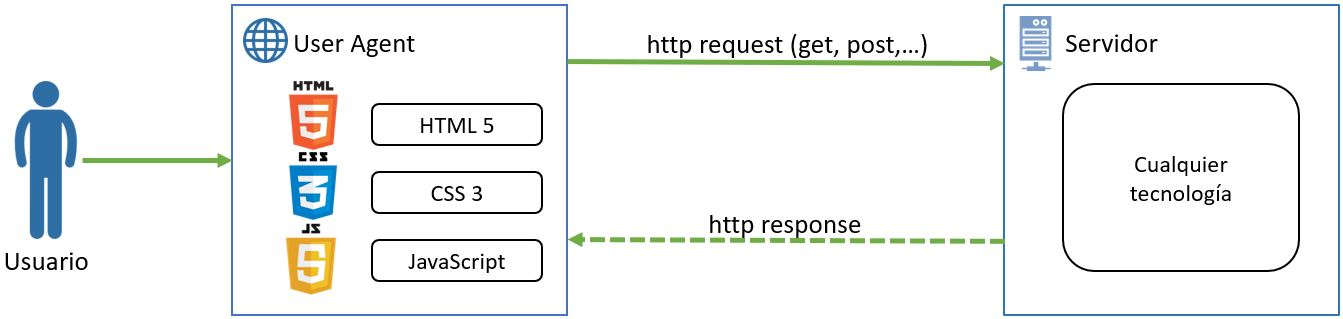
\includegraphics[width=1\textwidth]{comunicacionWeb}
\caption{Esquema de comunicación HTTP}
\label{fig:comunicacionWeb}
\end{center}
\end{figure} 

Otra forma habitual de comunicación entre cliente y servidor son los \emph{websockets} \cite{websockets}; no obstante, se omite su descripción ya que no se han utilizado para el desarrollo del proyecto.

\section{JHipster}
\label{sec:JHipster}

JHipster se trata de un framework de desarrollo rápido de aplicaciones web que, a partir de un fichero en el que se describe la estructura de datos del sistema, el JDL (JHipster Domain Language) \cite{jdl}, un motor de generación de código produce el código del cliente, el del servidor y el de la base de datos, generando una aplicación completamente funcional. 

\begin{wrapfigure}{r}{0.60\textwidth} %this figure will be at the right
    \centering
    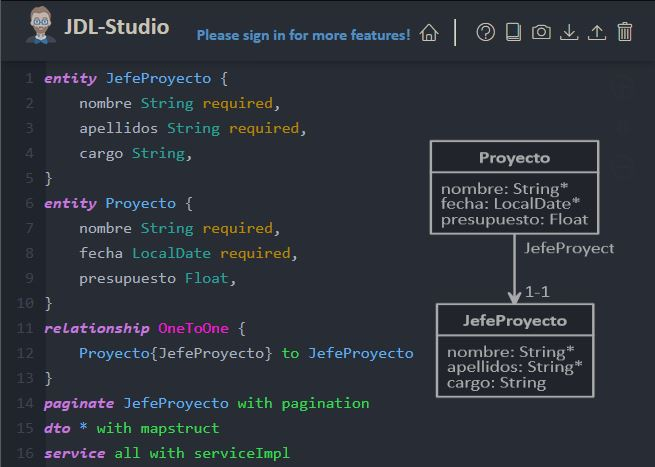
\includegraphics[width=0.60\textwidth]{jdlStudio}
    \caption{Ejemplo de JDL}
    \label{fig:jdlStudio}
\end{wrapfigure}

La figura \ref{fig:jdlStudio} muestra un ejemplo sencillo de un código JDL que describe una aplicación en la que un proyecto tiene un jefe de proyecto, visto en JDL-Studio \cite{jdl-studio}. Esta herramienta permite escribir el JDL, mostrando errores que pueda contener el código y generando en tiempo real un diagrama con la estructura de la aplicación. 

En el código le indicamos las entidades que habrá en la aplicación y sus atributos, las relaciones que hay entre ellos y además se le puede indicar si se desea que las entidades tengan paginación o si queremos o no que se generen los DTO (Data Transfer Object) o los \emph{ServicesImpl}, dónde está el negocio de la aplicación.

JDL-Studio ofrece además la posibilidad de gestionar los diferentes JDL con los que hayamos trabajado guardándolos en nuestra cuenta.

Por otro lado, permite exportar el código que hemos escrito o obtener una imagen del diagrama generado que se podrá usar para la documentación del proyecto, por ejemplo, como es el caso de este trabajo \ref{anex:1}.

Toda la documentación sobre el lenguaje está disponible en la misma herramienta de edición, siendo posible tener en la misma pantalla nuestro código, el diagrama de éste y la documentación para consultarla mientras escribimos.

A partir del código del JDL, JHipster genera:
\begin{itemize}
\item Para la parte del cliente: 

Todos los archivos que necesita Angular 5 (sección \ref{sec:Angular5}). Esto supone que generará el cliente siguiendo el patrón MVC (Modelo Vista Controlador) dentro del cliente que permitirá tratar los datos de manera similar a como lo haría una aplicación de escritorio. Se generarán para el Jefe y el Proyecto todos los HTML necesarios, con su detalle y diálogos, además del CSS necesario para su maquetación. 

Además, se generan diferentes archivos en \emph{TypeScript} para los diferentes componentes y sus servicios, que serán los encargados de la comunicación con el lado servidor.

\begin{figure}[!h]
\begin{center}
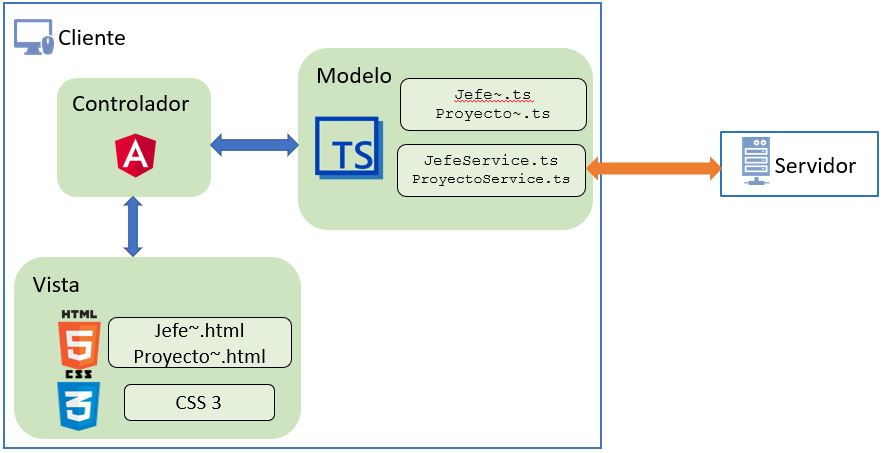
\includegraphics[width=1\textwidth]{ejemploCliente}
\caption{Cliente para el ejemplo de Jefes y Proyectos}
\label{fig:ejemploCliente}
\end{center}
\end{figure}
\clearpage

\item Para el servidor: 

Genera un MVC, los Resource que se encargan de la comunicación con el cliente, los Services en los que estará el negocio de la aplicación, y los repository que serán los que realicen operaciones sobre la base de datos. 

Los DTO se encargan de transmitir información entre \emph{Services} y \emph{Resources}, y las clases para cada entidad  lo harán con los \emph{Services} y los \emph{Repository}.

\begin{figure}[!h]
\begin{center}
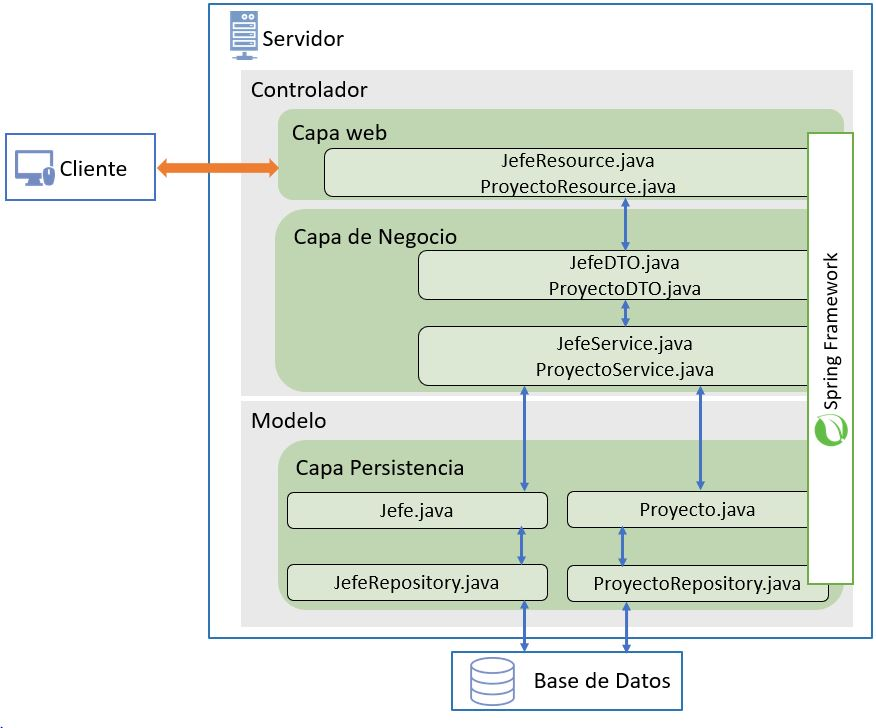
\includegraphics[width=1\textwidth]{ejemploServer}
\caption{Servidor para el ejemplo de Jefes y Proyectos}
\label{fig:ejemploServer}
\end{center}
\end{figure}

\item Finalmente, para la base de datos:

Cada clase es anotada con etiquetas como \emph{@Table} o \emph{@Column}, que servirá para generar un archivo \emph{xml} para cada entidad con su estructura en base de datos y otro con las relaciones entre entidades. Después, \emph{Liquibase}, que es una librería de gestión y aplicación de cambios en bases de datos \cite{liquibase}, se encarga de traducirlo al formato soportado por nuestra base de datos y crear o añadir los cambios en ella.

\begin{figure}[!h]
\begin{center}
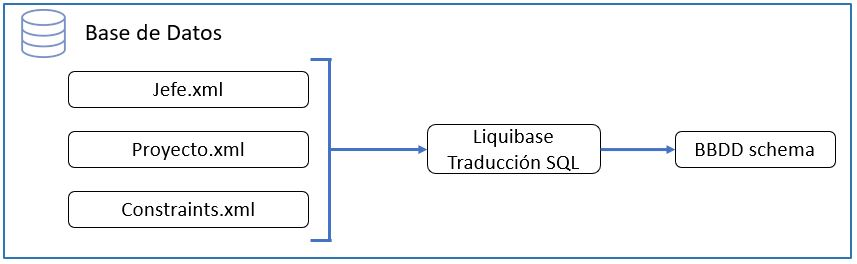
\includegraphics[width=0.75\textwidth]{ejemploBBDD}
\caption{Base de Datos para el ejemplo de Jefes y Proyectos}
\label{fig:ejemploBBDD}
\end{center}
\end{figure}

\end{itemize}

\section{Angular 5}
\label{sec:Angular5}

Angular (Figura \ref{fig:angularLogo}) se trata de un framework de desarrollo de aplicaciones web desarrollado por Google \cite{angular}, la versión 5 será la usada en ONCOSUP. El lenguaje usado es \emph{TypeScript}, en el que se generan los diferentes componentes, servicios o enrutadores. Angular trata de facilitar el desarrollo de aplicaciones web implementando un MVC en el front-end, que además facilita las pruebas.

\begin{wrapfigure}{r}{0.55\textwidth} %this figure will be at the right
    \centering
    
\includegraphics[width=0.55\textwidth]{angularLogo}
    \caption{Proyecto Angular}
    \label{fig:angularLogo}
\end{wrapfigure}
Angular es una tecnología con un despegue relativamente nuevo, pero su primera versión, AngujarJS, salió a la luz en el año 2010. Esta versión estaba limitada al uso de JavaScript, y su uso se fue popularizándose en el 2012 hasta que apareciera una nueva versión del framework. Angular fue, de alguna forma, una manera de impulsar el cambio de Apache y PHP a JavaScript tanto en el front-end como en el back-end.

En septiembre de 2016 se lanza la nueva versión de AngularJS, en la que pierde el JS y se empiezan a numerar, saliendo a la luz Angular 2. La segunda versión de Angular fue reescrita casi por completo, conservando conceptos de funcionalidad. El paso de AngularJS a Angular 2, supuso un descontento en la comunidad que había estado desarrollando sus aplicaciones con AngularJS, ya que ahora tendrían que volver a empezar sus proyectos o migrarlos de alguna manera a Angular 2. A pesar de esto, el cambio a la nueva versión supuso una mejora, ya que Google pretendía llevar una gestión de versiones que permitiera ir añadiendo funcionalidad, conservando la compatibilidad entre versiones.

Alrededor de seis meses después, en marzo de 2017, el equipo de Google lanza Angular 4, con diferencias no muy significativas respecto a la versión anterior, pero que conservaba retrocompatibilidad con la anterior. Esta nueva versión, al llegar tan rápido, causó revuelo en la comunidad, haciendo pensar a los usuarios del framework que ocurriría lo mismo que con el salto de Angular JS a Angular 2. Afortunadamente no fue así y la popularidad de la herramienta fue aumentando.

En noviembre de ese mismo año se publica Angular 5, versión que se usará para el desarrollo de ONCOSUP, que añadiría mejoras de rendimiento, junto con alguna funcionalidad nueva.

Durante el desarrollo del proyecto, en marzo de 2018, saldrá a la luz la nueva versión, Angular 6. Y se estima que Angular 7, será lanzado entre septiembre y noviembre del mismo año.

Como curiosidad, la versión Angular 3 nunca salió a la luz y se saltó directamente a la versión 4 debido a un desalineamiento con la numeración de las versiones de uno de sus paquetes que iban por su versión 3.



\section{Otras tecnologías}
\label{sec:otrasTec}

Algunas tecnologías que se usarán en el proyecto, pero en las que no se profundizará tanto, son (figura \ref{chap:antecedentes}):

\begin{itemize}
\item MariaDB \cite{mariaDB} - Se trata de una evolución de MySQL en la que han estado trabajando algunos de los desarrolladores originales de MySQL.
\item SpringBoot \cite{springBoot} - Herramienta de generación de código, que JHipster usa y añade nuevos elementos para crear una aplicación más completa que la que SpringBoot ofrece.
\item Spring Security \cite{springSec} - Toda la seguridad de la aplicación será gestionada por esta herramienta del framework de Spring. Los desarrolladores tan sólo tendrán que hacer pequeñas modificaciones para que se ajuste a las necesidades de la aplicación.
\item Apache Tomcat \cite{tomcat} - La generación de la aplicación incluye un servidor Tomcat embebido. 

\end{itemize}

\begin{figure}[!h]
\begin{center}

\includegraphics[width=1\textwidth]{otrasTecnologias}
\caption{Otras tecnologías que se usarán para el desarrollo del proyecto}
\label{fig:otrasTecnologias}
\end{center}
\end{figure}

% Local Variables:
%  coding: utf-8
%  mode: latex
%  mode: flyspell
%  ispell-local-dictionary: "castellano8"
% End:
